\documentclass[letterpaper,spanish,reprint,nofootinbib,showkeys,aps]{revtex4-2}

%%%%%%%%%%%%%%%%%%%%%%%%%%%%%%%%%%%%%%%%%%%%%%%%%%%%%%%%%%%%%%%%%%%%%%%%%%%%
% PAQUETES USUALES
\usepackage[T1]{fontenc}
\usepackage[utf8]{inputenc}
\usepackage[spanish]{babel} 
\usepackage{calc}
\usepackage{amsmath,bm,amssymb}
\usepackage{fancyhdr}
\usepackage{pythonhighlight}
\usepackage{graphicx}
\usepackage{float}\usepackage{xcolor}
%para escribir código%%%%%%%%%%%%%%
\usepackage{algorithm}
\usepackage{algpseudocode}
\usepackage{listings}
\usepackage{color, xcolor}
%%%Algunos comandos útiles para el PDF generado%%%
\usepackage[unicode=true,pdfusetitle, bookmarks=true,bookmarksnumbered=false,bookmarksopen=false, breaklinks=false,pdfborder={0 0 1},backref=false,colorlinks=true] {hyperref}
\hypersetup{
 citecolor=dkgreen,linkcolor=blue,urlcolor=blue}
%%% PARA TEOREMAS NUEVOS
\usepackage{amsthm}
\renewcommand{\qedsymbol}{\tiny{$\blacksquare$}}
\newenvironment{solucion}{\begin{proof}[\textcolor{magenta}{Solución}]}{\end{proof}}
\usepackage{mdframed}
\usepackage[many]{tcolorbox}
\usepackage{thmtools}


%%%%%%%%%%%%%%%%%%%%%%%%%%%%%%%%%%%%%%%%%%%%%%%%%%%%%%%%%%%%%%%%%%%%%%%%%%%%
%%%%%%%%%%%%%%%%%%%%%%%%%%%%%%%%%%%%%%%%%%%%%%%%%%%%%%%%%%%%%%%%%%%%%%%%%%%%
%%%%%%%%%%%%%%%%%%%%%%%%%%%% MARGENES %%%%%%%%%%%%%%%%%%%%%%%%%%%%%%%%%%%%%%
%%%%%%%%%%%%%%%%%%%%%%%%%%%%%%%%%%%%%%%%%%%%%%%%%%%%%%%%%%%%%%%%%%%%%%%%%%%%
%%%%%%%%%%%%%%%%%%%%%%%%%%%%%%%%%%%%%%%%%%%%%%%%%%%%%%%%%%%%%%%%%%%%%%%%%%%%

\parskip=5pt
\hoffset = 0pt
\headsep = 0.8 cm % estaba en 1.5 cm, lo cambie para el header de la imagen
\setlength{\parindent}{0cm}

%%%%%%%%%%%%%%%%%%%%%%%%%%%%%%%%%%%%%%%%%%%%%%%%%%%%%%%%%%%%%%%%%%%%%%%%%%%%
%%%%%%%%%%%%%%%%%%%%%%%%%%%%%%%%%%%%%%%%%%%%%%%%%%%%%%%%%%%%%%%%%%%%%%%%%%%%
%%%%%%%%%%%%%%%%%%%%%%%%% EJERRCICIOS  %%%%%%%%%%%%%%%%%%%%%%%%%%%%%%%%%%%%%
%%%%%%%%%%%%%%%%%%%%%%%%%%%%%%%%%%%%%%%%%%%%%%%%%%%%%%%%%%%%%%%%%%%%%%%%%%%%
%%%%%%%%%%%%%%%%%%%%%%%%%%%%%%%%%%%%%%%%%%%%%%%%%%%%%%%%%%%%%%%%%%%%%%%%%%%%

\newtcolorbox[auto counter,number within=section]{ejercicio}[1][]{
% ESTO ES PARA LA CAJA GENERAL
breakable, % por si cambias de pagina
enhanced, % estilo general
% TITULO MODIFICACIONES
coltitle= black,
colbacktitle= white,
titlerule= 0mm,
colframe = magenta,
fonttitle=\bfseries,
title= Ejercicio~\thetcbcounter,
% CAJA LINEA MODIFICACIONES
boxed title style={
  sharp corners,
  rounded corners=northwest,
  rounded corners=northeast,
  % outer arc=0pt,
  % arc=0pt,
  },
% CONTENIDO MODIFICACIONES
colback = white,
fontupper = \itshape,
coltext =  black,
% MARCO MODIFICACIONES
rightrule=0mm,
toprule=0pt,
bottomrule= 0pt,
leftrule = 4pt
}

%%%%%%%%%%%%%%%%%%%%%%%%%%%%%%%%%%%%%%%%%%%%%%%%%%%%%%%%%%%%%%%%%%%%%%%%%%%%
%%%%%%%%%%%%%%%%%%%%%%%%%%%%%%%%%%%%%%%%%%%%%%%%%%%%%%%%%%%%%%%%%%%%%%%%%%%%
%%%%%%%%%%%%%%%%%%%%%%%%% MEMO PYTHON Y C %%%%%%%%%%%%%%%%%%%%%%%%%%%%%%%%%%
%%%%%%%%%%%%%%%%%%%%%%%%%%%%%%%%%%%%%%%%%%%%%%%%%%%%%%%%%%%%%%%%%%%%%%%%%%%%
%%%%%%%%%%%%%%%%%%%%%%%%%%%%%%%%%%%%%%%%%%%%%%%%%%%%%%%%%%%%%%%%%%%%%%%%%%%%


\definecolor{dkgreen}{rgb}{0.9,0.6,0.8}
\definecolor{blue}{rgb}{0.0,0.49,0.4}
\definecolor{gray97}{gray}{.97}
\definecolor{gray75}{gray}{.75}
\definecolor{gray45}{gray}{.45}
\definecolor{codegreen}{rgb}{0,0.6,0}
\definecolor{codegray}{rgb}{0.5,0.5,0.5}
\definecolor{codepurple}{rgb}{0.58,0,0.82}
\definecolor{backcolour}{rgb}{0.95,0.95,0.92}

\lstdefinestyle{mystyle}{
    backgroundcolor=\color{gray97},
    commentstyle=\color{cyan!75!black},
    keywordstyle=\color{magenta},
    numberstyle=\tiny\color{codegray},
    stringstyle=\color{codepurple},
    basicstyle=\ttfamily\footnotesize,
    breakatwhitespace=false,
    breaklines= true,
    captionpos=b,
    keepspaces=true,
    numbers=left,
    numbersep=5pt,
    showspaces=false,
    showstringspaces=false,
    showtabs=false,
    tabsize=2,
    language=bash,   %% PHP, C, Java, etc... bash is the standard
    extendedchars=true,
    inputencoding=latin1
}

\lstset{style=mystyle, literate =
                        {í}{{\'i}}1
                        {á}{{\'a}}1
                        {é}{{\'e}}1
                        {ó}{{\'o}}1
                        {ú}{{\'u}}1
                        {ñ}{{\~n}}1
                        {ü}{{\"u}}1
                            }

%%%%%%%%%%%%%%%%%%%%%%%%%%%%%%%%%%%%%%%%%%%%%%%%%%%%%%%%%%%%%%%%%%%%%%%%%%%%
%%%%%%%%%%%%%%%%%%%%%%%%%%%%%%%%%%%%%%%%%%%%%%%%%%%%%%%%%%%%%%%%%%%%%%%%%%%%
%%%%%%%%%%%%%%%%%%%%% ##ENCABEZADOS Y NUMERACION %%%%%%%%%%%%%%%%%%%%%%%%%%%%%
%%%%%%%%%%%%%%%%%%%%%%%%%%%%%%%%%%%%%%%%%%%%%%%%%%%%%%%%%%%%%%%%%%%%%%%%%%%%
%%%%%%%%%%%%%%%%%%%%%%%%%%%%%%%%%%%%%%%%%%%%%%%%%%%%%%%%%%%%%%%%%%%%%%%%%%%%

\pagestyle{fancy}
\fancyhf{}
\fancyfoot{\thepage}
\fancyfoot[R]{\small{\textsc{Sarahi García, Ramón Ruíz}}}
\fancyfoot[L]{\small{\textsc{Reconocimiento estadístico de patrones}}}
\chead{\includegraphics[scale=.27]{/Users/ely/Documents/Plantilla/Figures/waves.pdf}}
\renewcommand{\headrulewidth}{0pt}
\renewcommand{\footrulewidth}{0pt}

%%%%%%%%%%%%%%%%%%%%%%%%%%%%%%%%%%%%%%%%%%%%%%%%%%%%%%%%%%%%%%%%%%%%%%%%%%%%
%%%%%%%%%%%%%%%%%%%%%%%%%%%%%%%%%%%%%%%%%%%%%%%%%%%%%%%%%%%%%%%%%%%%%%%%%%%%
%%%%%%%%%%%%%%%%%%%%%%%%%%%%%%%%%%%%%%%%%%%%%%%%%%%%%%%%%%%%%%%%%%%%%%%%%%%%
%%%%%%%%%%%%%%%%%%%%%%%%%%%%%%%%%%%%%%%%%%%%%%%%%%%%%%%%%%%%%%%%%%%%%%%%%%%%

%%%Declaración de operadores%%%
\DeclareMathOperator{\sech}{sech}

%%%%%%%%%%%%%%%%%%%%%%%%%%%%%%%%%%%%%%%%%%%%%%%%%%%%%%%%%%%%%%%%%%%%%%%%%%%%
%%%%%%%%%%%%%%%%%%%%%%%%%%%%%%%%%%%%%%%%%%%%%%%%%%%%%%%%%%%%%%%%%%%%%%%%%%%%
%%%%%%%%%%%%%%%%%%%%%%%%%%%%%%%%%%%%%%%%%%%%%%%%%%%%%%%%%%%%%%%%%%%%%%%%%%%%
%%%%%%%%%%%%%%%%%%%%%%%%%%%%%%%%%%%%%%%%%%%%%%%%%%%%%%%%%%%%%%%%%%%%%%%%%%%%


\begin{document}

\preprint{Reconocimiento estadístico de patrones}
\title{\Large{\textbf{Estudio de INP en México}}}
%\thanks{A footnote to the article title}
\author{Sarahi García, Ramón Ruíz}
\email{yesenia.garcia@cimat.mx, ramon.ruiz@cimat.mx}
\affiliation{\vspace{0.15cm}Centro de Investigación en Matemáticas CIMAT}
\thanks{REP, a  cargo de Dr. Johan Van horebeek}


%%%%%%%%%%%%%%%%%%%%%%%%%%%%%%%%%%%%%%%%%%%%%%%%%%%%%%%%%%%%%%%%%%%%%%%%%%%%
%%%%%%%%%%%%%%%%%%%%%%%%%%%%%%%%%%%%%%%%%%%%%%%%%%%%%#0Abstract%%%%%%%%%%%%%%%
%%%%%%%%%%%%%%%%%%%%%%%%%%%%%%%%%%%%%%%%%%%%%%%%%%%%%%%%%%%%%%%%%%%%%%%%%%%%
%%%%%%%%%%%%%%%%%%%%%%%%%%%%%%%%%%%%%%%%%%%%%%%%%%%%%%%%%%%%%%%%%%%%%%%%%%%%

\begin{abstract}
\begin{center}
\small{15 de Abril de 2024}
\end{center}
\vspace{0.6cm}


En este trabajo, realizamos visualización y análisis de datos multidimensionales de los precios de algunos productos que proporciona una las herramientas del INPC del INEGI. Generamos una pequeña base datos con productos específicos, incluyendo limón, leche, camarón, tortillas, electricidad, alquiler, frijol y pollo, en el perido Agosto-2018 a Febrero-2024. Aplicamos análisis de componentes principales (PCA) para reducir la dimensionalidad de los datos y proyectarlos en un espacio tridimensional. Luego, empleamos el algoritmo K-means para agrupar los datos en un número predeterminado de clusters. Posteriormente, generamos histogramas para cada variable en función de los clusters obtenidos, lo que permite explorar la distribución de los datos dentro de cada cluster. Pudimos observar una cierta estructura en los datos relacionada con el año y el tipo de ciudad al que pertenecen.


\end{abstract}

\maketitle

%%%%%%%%%%%%%%%%%%%%%%%%%%%%%%%%%%%%%%%%%%%%%%%%%%%%%%%%%%%%%%%%%%%%%%%%%%%%
%%%%%%%%%%%%%%%%%%%%%%%%%%%%%%%%%%%%%%%%%%%%%%%%%%%#1INTRODUCION%%%%%%%%%%%%%
%%%%%%%%%%%%%%%%%%%%%%%%%%%%%%%%%%%%%%%%%%%%%%%%%%%%%%%%%%%%%%%%%%%%%%%%%%%%



\section{Introducción}



El Índice Nacional de Precios al Consumidor (INPC) es un indicador de la evaluación y comprensión de la dinámica económica del país. Esta diseñado para estimar la evolución de los precios de los bienes y servicios consumidos por las familias de México.

Existe una complejidad inherente a la medición de las variaciones de precios pues, entre otros factores, existe una amplia gama de artículos y servicios de consumo así como una constante fluctuación en los precios. Además, la asincronía en los cambios de precios y sus variaciones de velocidad agregan un nivel adicional de complejidad al análisis.

En este contexto, el presente se enfoca en analizar los precios de una amplia gama de productos en diversas ciudades de México. Utilizando datos muestrales, exploramos las fluctuaciones en los precios de nueve productos a lo largo del tiempo y en diferentes ubicaciones geográficas del país. Empleamos técnicas de análisis estadístico y visualización de datos para identificar patrones y relaciones significativas en los datos.

La información recopilada para este análisis proviene de la base de datos proporcionada por una de las herramientas de del INPC del INEGI: \textbf{Consulta precios promedio}, que contiene registros de precios de distintas marcas y/o proovedores de una serie de productos y servicios en 55 ciudades que se consumen en todo el país. Las cotizaciones de los productos en esta base de datos son principalmente mensuales y se encuentran desde el mes de Agosto del año 2018.

Hay una extensa cantidad de productos y servicios disponibles en la página del INEGI, pero nosotros nos centraremos exclusivamente en los siguientes productos mostrados en \ref{res}, desde el mes de agosto de 2018 hasta el mes de marzo de 2024 de las 55 ciudades. Para un mejor manejo y representación visual de los datos se modificaron, y/o quitaron
algunas de las filas, de modo que para cada producto/servicio tenemos un único proveedor/marca. 

El procedimiento de cómo llegamos a esta única tabla de datos se encuentra en el notebook \texttt{preprocesamiento.ipynb}, en \ref{res} se encuentra una pequeña tabla con la info de las variables que utilizaremos.


\begin{figure} [H]
	\begin{center}
		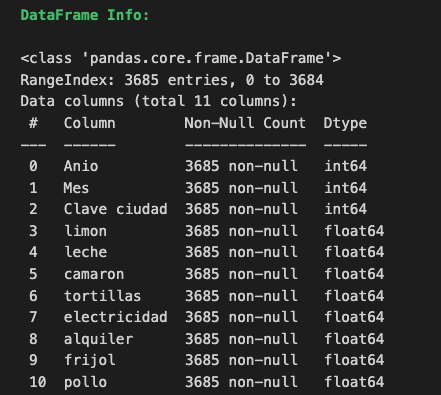
\includegraphics[scale=0.38]{/Users/ely/Documents/Maestria/segundo_semestre/cimat2023-1/patrones/Proyecto_1/imgenes/resumen.png}
		\caption{DataFrame Info}
		\label{res} 
   \end{center} 
\end{figure}


\section{Análisis Exploratorio }

\subsection*{Productos}

Sobre las variables continuas y cuantitativas (los precios de cada producto), algunas de las características que nos interesan son su promedio, media, máximo, mínimo, etc, que se muestra en la tabla \ref{sts}. 

\begin{figure} [H]
	\begin{center}
		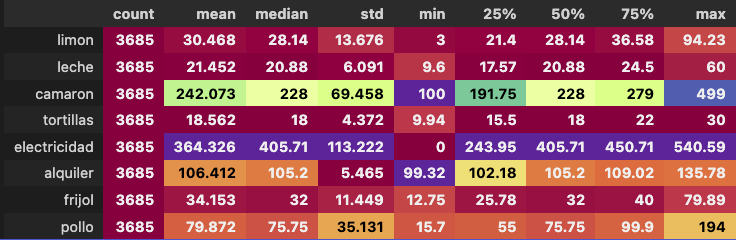
\includegraphics[scale=0.3]{/Users/ely/Documents/Maestria/segundo_semestre/cimat2023-1/patrones/Proyecto_1/imgenes/sts.png}
		\caption{DataFrame Info}
		\label{sts} 
   \end{center} 
\end{figure}

Estas estadísticas son sobre el total de datos, es decir, toma en cuenta todas las ciudades, y todos los meses de los 4 años. Más adelante veremos unos gráficos para ciertas ciudades y/o a lo largo del tiempo.

El limón, el frijol, la leche, el alquiler siguen una distribución unimodal y presentan una asimetría hacia la derecha. A continuación se muestran el histograma y boxplot del limon \ref{limon} y el alquiler \ref{alquiler}.

\begin{figure} [H]
	\begin{center}
		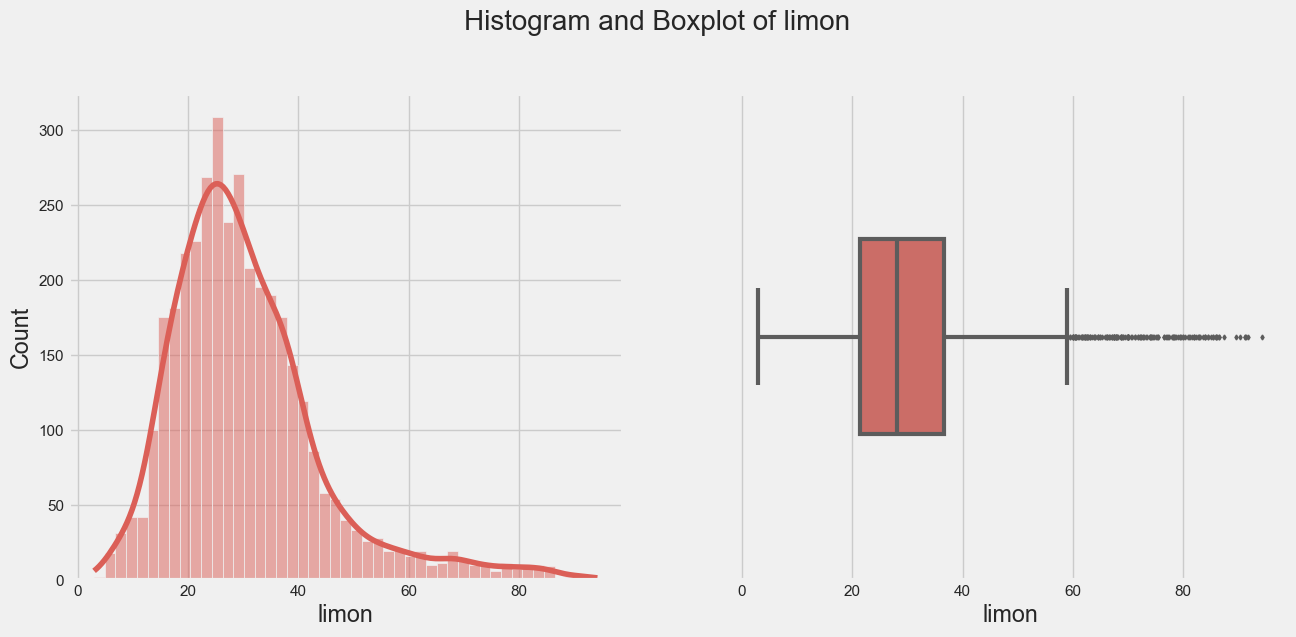
\includegraphics[scale=0.24]{/Users/ely/Documents/Maestria/segundo_semestre/cimat2023-1/patrones/Proyecto_1/imgenes/hblimon.png}
		\caption{Histograna y Boxplot de precios del Limón }
		\label{limon} 
   \end{center} 
\end{figure}

\begin{figure} [H]
	\begin{center}
		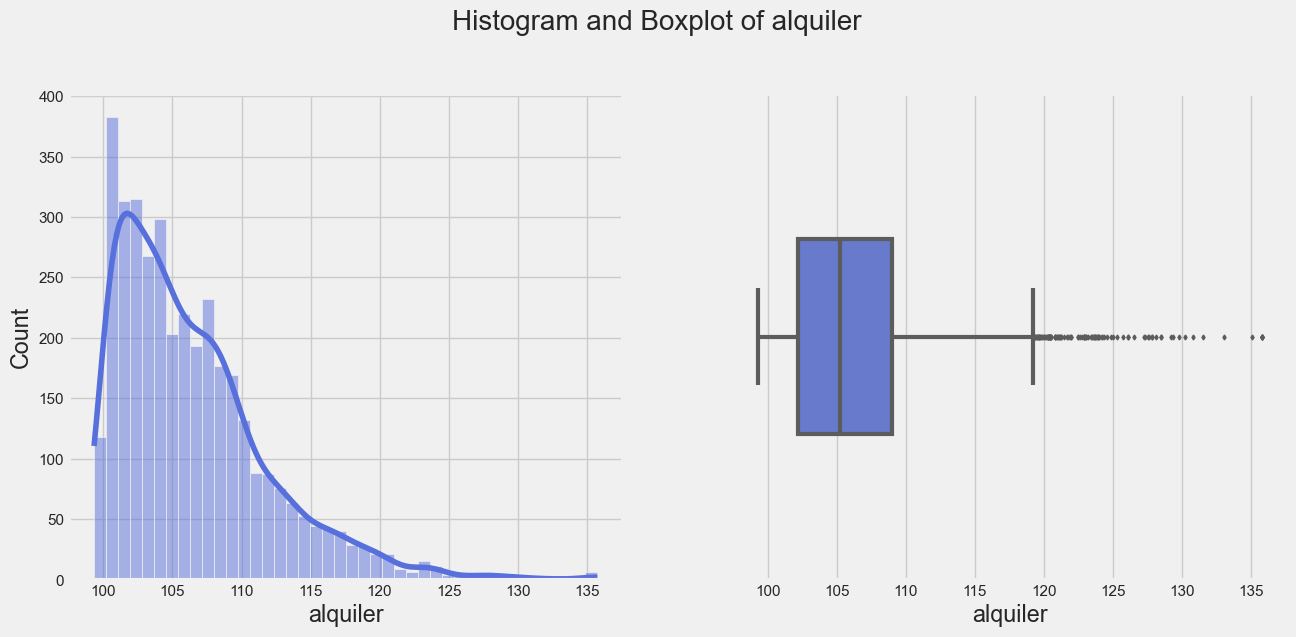
\includegraphics[scale=0.24]{/Users/ely/Documents/Maestria/segundo_semestre/cimat2023-1/patrones/Proyecto_1/imgenes/hbalquiler.png}
		\caption{Histograna y Boxplot de precios del alquiler }
		\label{alquiler} 
   \end{center} 
\end{figure}


El camarón presenta una distribución bimodal \ref{camaron} y los demás productos (electricidad tortillas pollo) presentan distribuciones con una gran varianza (veáse tabla \ref{sts}), por ejemplo, en el caso de las tortillas \ref{tortillas}, el precio mínimo es de 9.94, el máximo es 30 y su desviación es 4.37, aproximadamente de un quinto del rango.

\begin{figure} [H]
	\begin{center}
		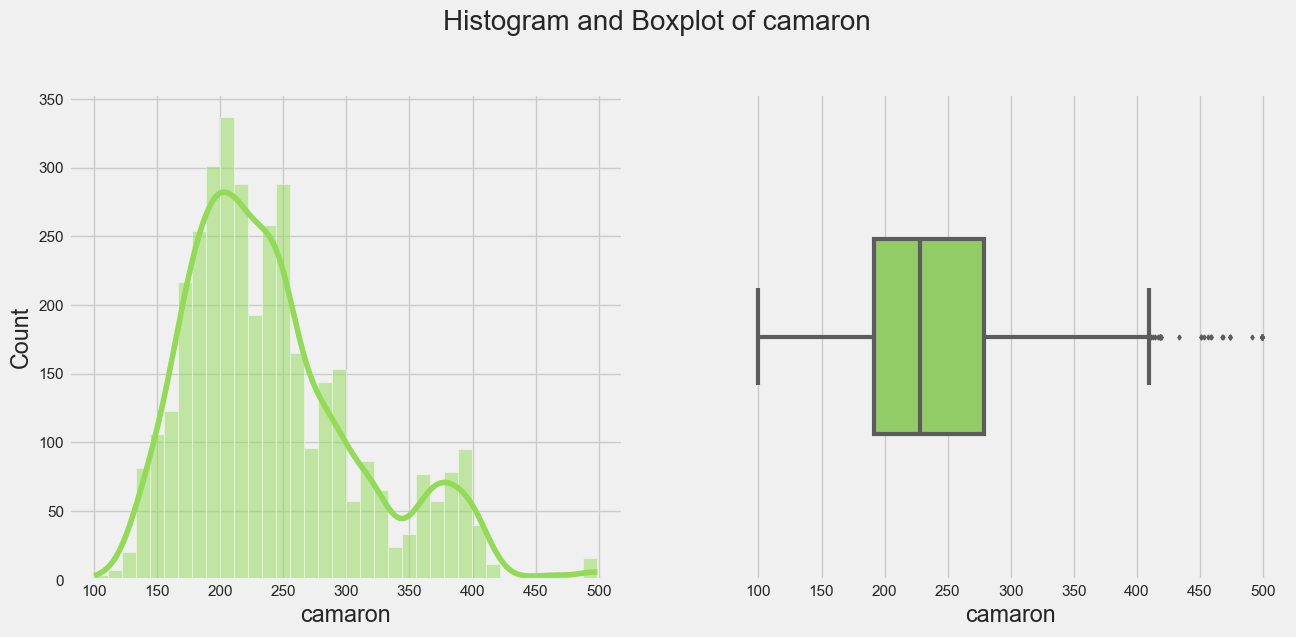
\includegraphics[scale=0.24]{/Users/ely/Documents/Maestria/segundo_semestre/cimat2023-1/patrones/Proyecto_1/imgenes/hbcamaron.png}
		\caption{Histograna y Boxplot de precios del camaron }
		\label{camaron} 
   \end{center} 
\end{figure}

\begin{figure} [H]
	\begin{center}
		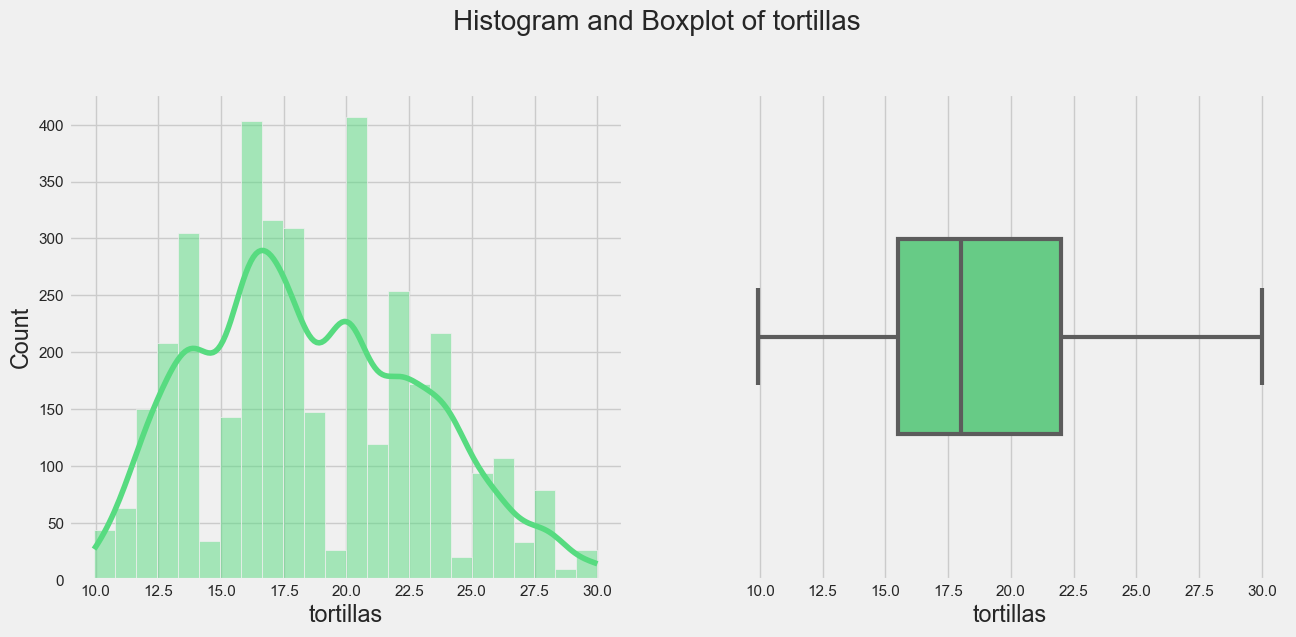
\includegraphics[scale=0.24]{/Users/ely/Documents/Maestria/segundo_semestre/cimat2023-1/patrones/Proyecto_1/imgenes/hbtortillas.png}
		\caption{Histograna y Boxplot de precios del tortillas }
		\label{tortillas} 
   \end{center} 
\end{figure}

Los demás histogramas y boxplots pueden consultarse en el notebook \texttt{analisis$\_$exploratorio.ipynb}.

\subsection*{Precios en el tiempo}


Otra caracteristica interesante sobre los precios de los distintos productos es su evolución en el tiempo. Los siguientes cuatro gráficos muestran esto para cada ciudad. 
En general, el rango de los precios en función de las ciudades (para un punto fijo en el tiempo) es grande a excepción del limón y la electricidad.

En estas dos imágenes podemos apreciar que todas las gráficas (cada una asociada a una cd. distinta) siguen un patrón bastante definido.


El precio del limón \ref{stlimon} tiene un máximo y un mínimo globales bien definidos por año y sólo unas cuantas ciudades no se apegan a este comportamiento. 

Mientras que el precio de la electriccidad \ref{stelectricidad} alcanza un mínimo y luego un máximo de manera periódica, además en estos precios se mantiene por tiempo para volver a subir o bajar después. 


\begin{figure} [H]
	\begin{center}
		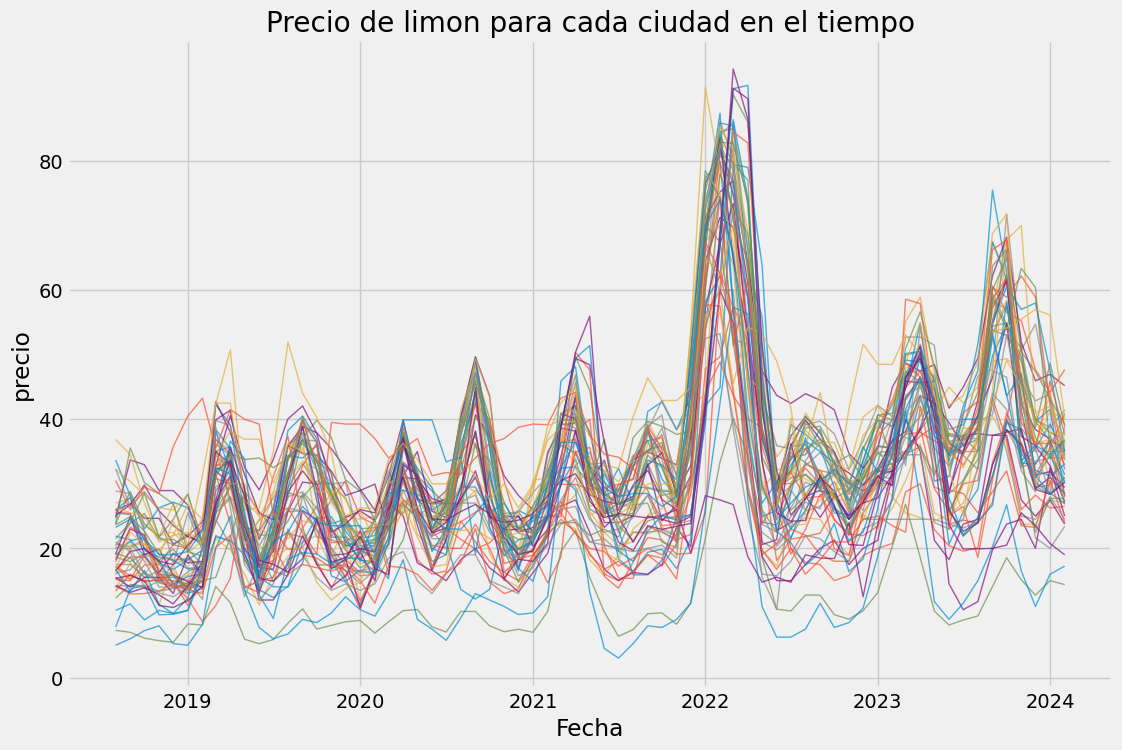
\includegraphics[scale=0.24]{/Users/ely/Documents/Maestria/segundo_semestre/cimat2023-1/patrones/Proyecto_1/imgenes/stlimon.png}
		\caption{Grafico de la variación de precios del limon para cada ciudad en el periodo agosto de 2018 a fenrero de 2024}
		\label{stlimon} 
   \end{center} 
\end{figure}


\begin{figure} [H]
	\begin{center}
		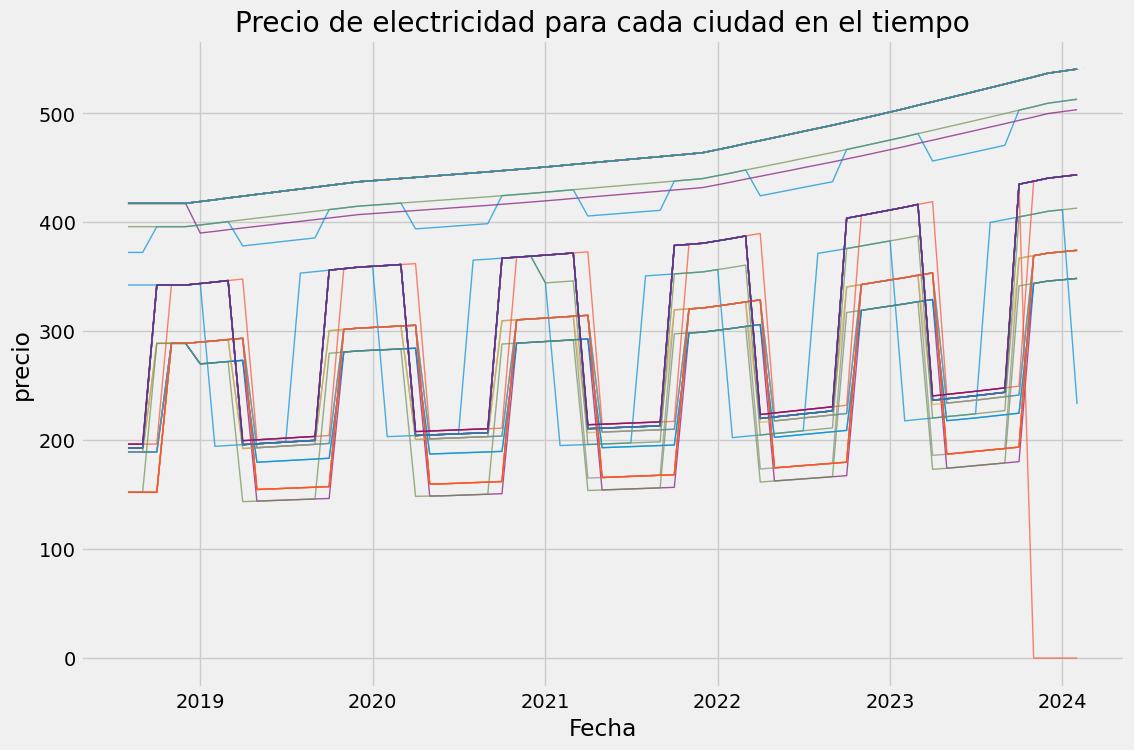
\includegraphics[scale=0.24]{/Users/ely/Documents/Maestria/segundo_semestre/cimat2023-1/patrones/Proyecto_1/imgenes/stelectricidad.png}
		\caption{Grafico de la variación de precios del electricidad para cada ciudad en el periodo agosto de 2018 a fenrero de 2024}
		\label{stelectricidad} 
   \end{center} 
\end{figure}

Un caso especial es el del alquiler donde también se muestra una tendencia similar en todas las ciudades, pareciera que los precios suben de manera msomenos lineal y las gráficas parecen no decrecientes. Sin embargo, a diferencia del limón y la electricidad, a medida que avanza el tiempo el rango de precios (en función de las ciudades y a tiempo fijo) es más grande. 

\begin{figure} [H]
	\begin{center}
		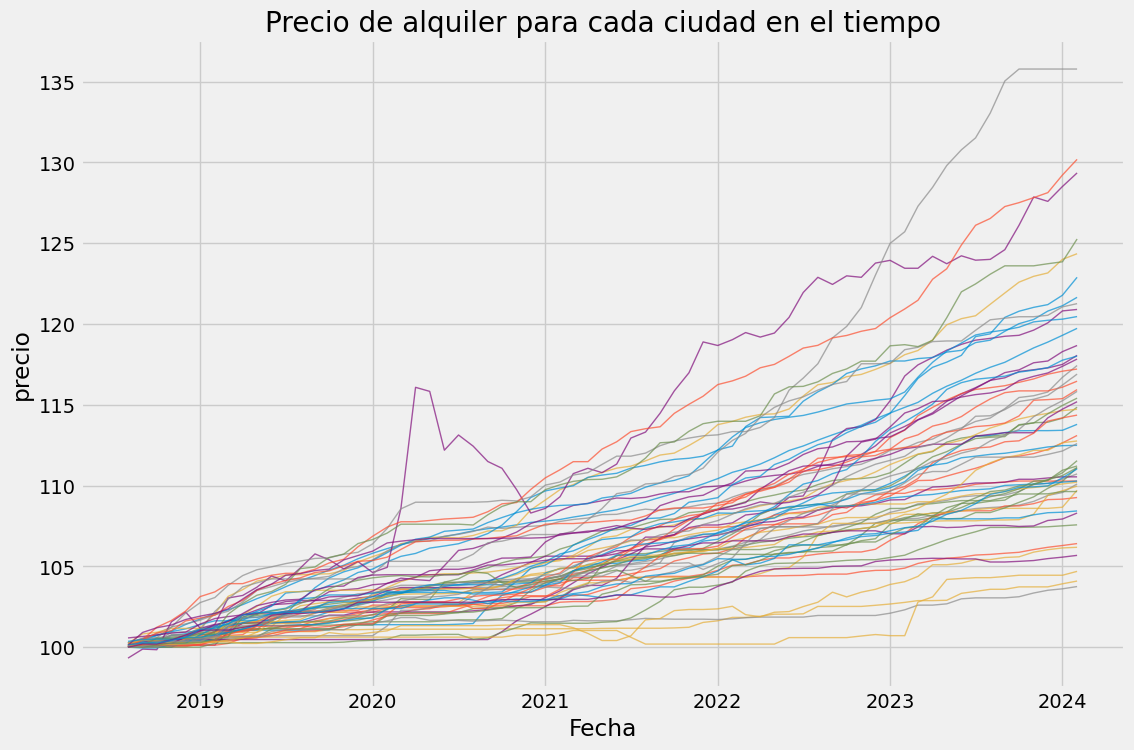
\includegraphics[scale=0.24]{/Users/ely/Documents/Maestria/segundo_semestre/cimat2023-1/patrones/Proyecto_1/imgenes/stalquiler.png}
		\caption{Grafico de la variación de precios del alquiler para cada ciudad en el periodo agosto de 2018 a fenrero de 2024}
		\label{stalquiler} 
   \end{center} 
\end{figure}

Como mencioamos antes, el rango de precios en ls distintas ciudades de los demás productos es bastante amplio en todo momento y su evolución no parece seguir ningún patrón en conjunto. Como ejemplo de estos casos, se muestra el gráfico de las tortillas \ref{sttortillas}.

\begin{figure} [H]
	\begin{center}
		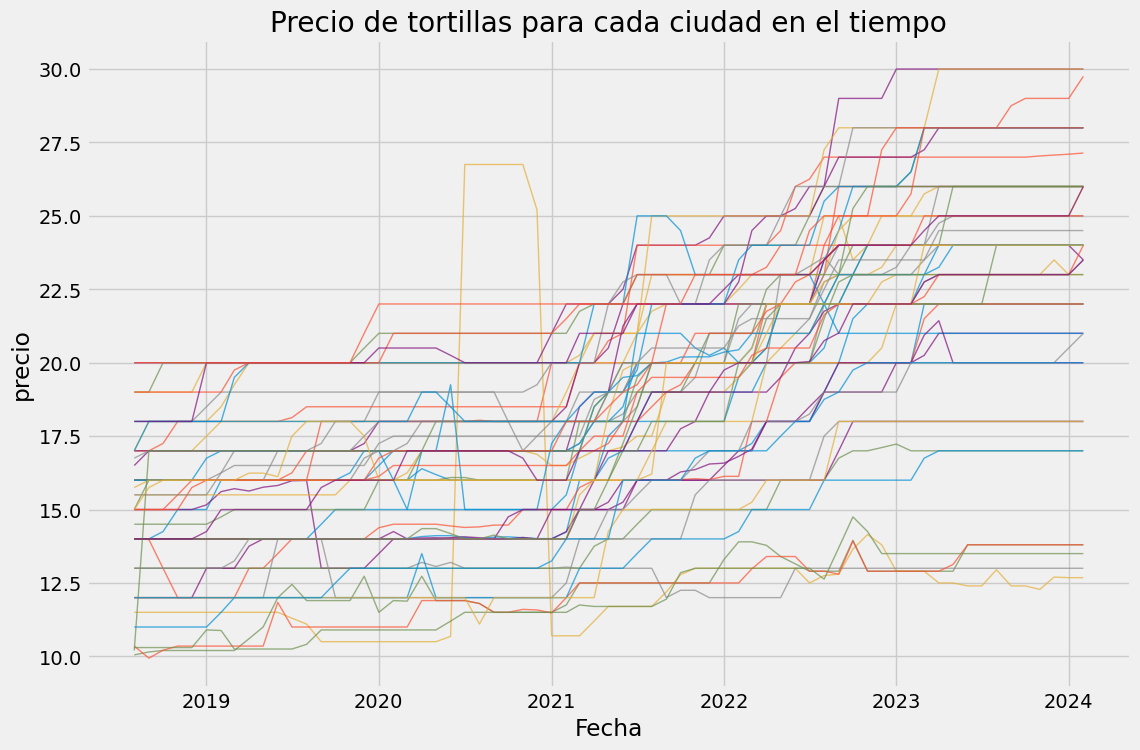
\includegraphics[scale=0.27]{/Users/ely/Documents/Maestria/segundo_semestre/cimat2023-1/patrones/Proyecto_1/imgenes/sttortillas.png}
		\caption{Grafico de la variación de precios del tortillas para cada ciudad en el periodo agosto de 2018 a fenrero de 2024}
		\label{sttortillas} 
   \end{center} 
\end{figure} 

Las demás series (pollo, camarón, leche y frijol) de tiempo tienen un comportamiento anpalogo al de las tortilla y pueden consultarse en el notebook \texttt{analisis$\_$exploratorio.ipynb}.

\subsection*{Ciudades}

Con los datos disponibles se realizó un resumen obteniendo el promedio de los precios de cada producto agrupando por ciudad (es decir, tomando en cuenta todos los meses de los 4 años para cada ciudad) y sumando estos valores se categorizó a cada ciudad en Caro, Medio o Barato. Se determino si una ciudad pertenecía o no a una categoría usando como referencia los cuantiles de la suma antes mencionada. 

\begin{figure} [H]
	\begin{center}
		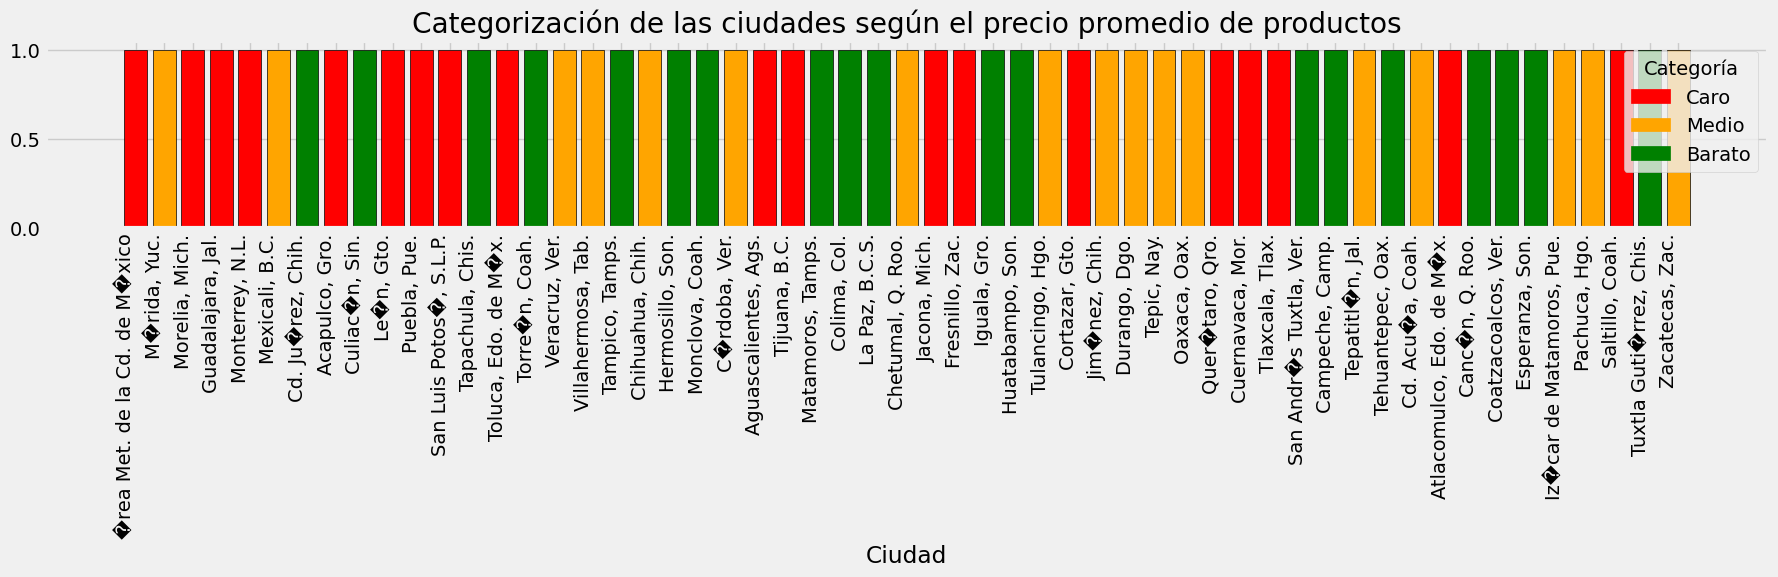
\includegraphics[scale=0.18]{/Users/ely/Documents/Maestria/segundo_semestre/cimat2023-1/patrones/Proyecto_1/imgenes/ciudades.png}
		\caption{Grafico de la variación de precios del ciudades para cada ciudad en el periodo agosto de 2018 a fenrero de 2024}
		\label{ciudades} 
   \end{center} 
\end{figure} 

Podemos ver que entre las ciudades más costosas se encuentran algunas como la Ciudad de México, Guadalajara, Monterrey, entre otras ciudades grandes y entre las ciudades más baratas tenemos ciudades más pequeñas como Huatabampo, La Paz, Campeche, Colima, etc. Las categorías asignadas coinciden con las que se podrían esperar dadas las naturalezas de las respectivas ciudades y sus estilos de vida.

Esta clasificación se agregó como variable categórica a nuestra base de datos para realizar algunas pruebas de clustering más adelante. 

\section{Resultados}

Buscamos alguna clasificación de los datos que pueda ayudarnos a discernir alguna estructura en estos por lo que comenzamos definiendo un vector aleatorio con los precios de los 8 productos y 4 variables aleatorias discretas, una por cada etiqueta disponible en nuestra base de datos: Año, Estación, Mes y Categoria. (Categoria se refiere a la clasificación de la ciudad \ref{ciudades})
\begin{figure} [H]
	\begin{center}
		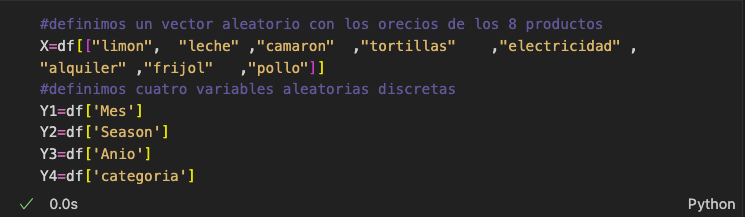
\includegraphics[scale=0.32]{/Users/ely/Documents/Maestria/segundo_semestre/cimat2023-1/patrones/Proyecto_1/imgenes/va.png}
		\caption{Variables aleatorias para realizar PCA y k-means}
		\label{va} 
   \end{center} 
\end{figure} 

Aplicamos PCA al vector aleatorio X y graficamos los datos proyectados en las primeras tres componentes principales, coloreando los datos de acuerdo al año \ref{pcaanio}, al mes \ref{pcames}, a la categoria \ref{pcacategoria} y a la estación del año \ref{pcaseason}.


\begin{figure} [H]
	\begin{center}
		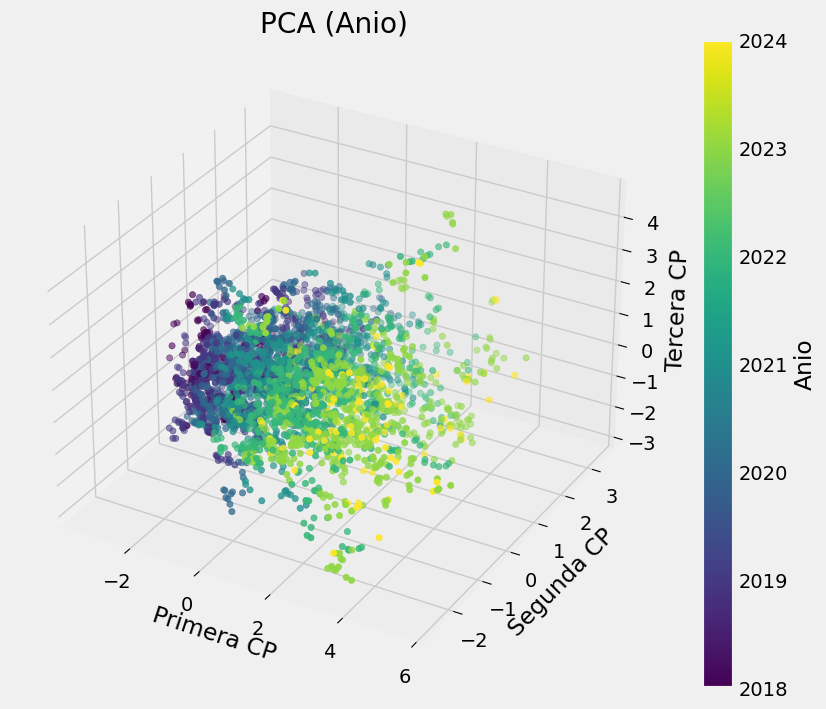
\includegraphics[scale=0.3]{/Users/ely/Documents/Maestria/segundo_semestre/cimat2023-1/patrones/Proyecto_1/imgenes/pcaanio.png}
		\caption{Primeras tres componentes principales coloreadas por año.}
		\label{pcaanio} 
   \end{center} 
\end{figure} 

En la gráfica de PCA año se aprecia un gradiente de color donde cada color representa un año, es decir, tenemos cierta estructura de acuerdo al año.



\begin{figure} [H]
	\begin{center}
		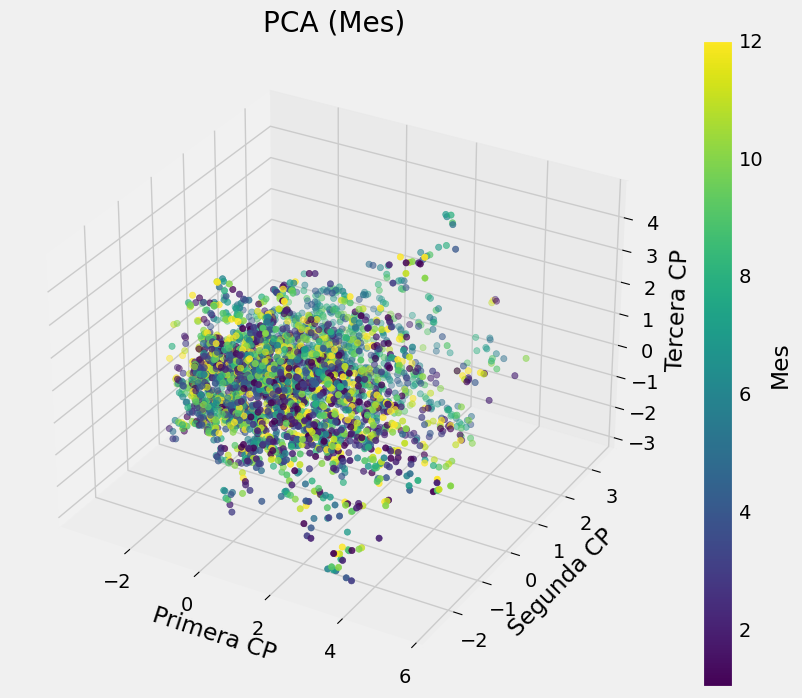
\includegraphics[scale=0.3]{/Users/ely/Documents/Maestria/segundo_semestre/cimat2023-1/patrones/Proyecto_1/imgenes/pcames.png}
		\caption{Primeras tres componentes principales coloreadas por mes.}
		\label{pcames} 
   \end{center} 
\end{figure} 



\begin{figure} [H]
	\begin{center}
		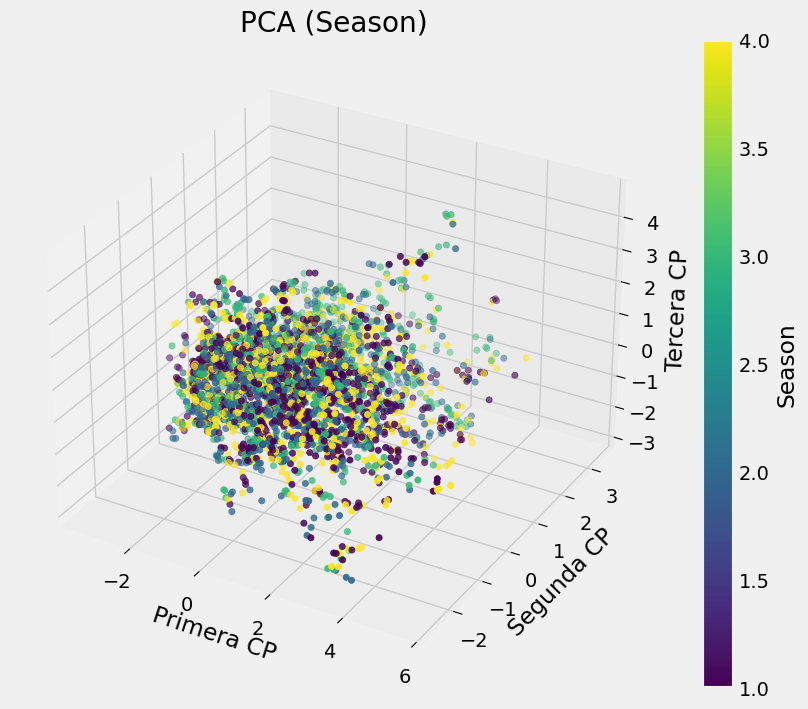
\includegraphics[scale=0.3]{/Users/ely/Documents/Maestria/segundo_semestre/cimat2023-1/patrones/Proyecto_1/imgenes/pcaseason.png}
		\caption{Primeras tres componentes principales coloreadas por estación.}
		\label{pcaseason} 
   \end{center} 
\end{figure} 


En los dos gráficos anteriores no se observa a simle vista ningún patrón bien definido como en el caso del año.

\begin{figure} [H]
	\begin{center}
		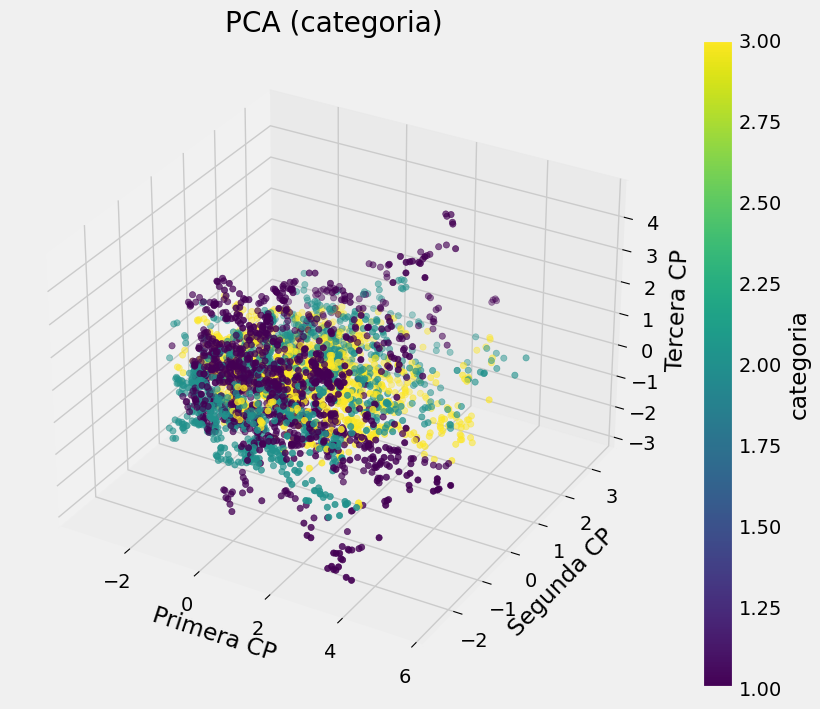
\includegraphics[scale=0.3]{/Users/ely/Documents/Maestria/segundo_semestre/cimat2023-1/patrones/Proyecto_1/imgenes/pcacategoria.png}
		\caption{Primeras tres componentes principales coloreadas por categoria (caro, barato, medio).}
		\label{pcacategoria} 
   \end{center} 
\end{figure} 

Finalmente, al colorear con las etiquetas de la variable categoría parece haber algo de agrupamiento, aunque desde el ángulo en que está la imagen no se aprecia adecuadamente.

En el notebook \texttt{pca$\_$clustering.ipynb} se encuentran además los gráficos de en 2D de las primeras dos componentes principales y otros gráficos 3D interactivos donde pueden apreciarse más detalladamente los datos y los colores de acuerdo al hue. 



\begin{figure} [H]
	\begin{center}
		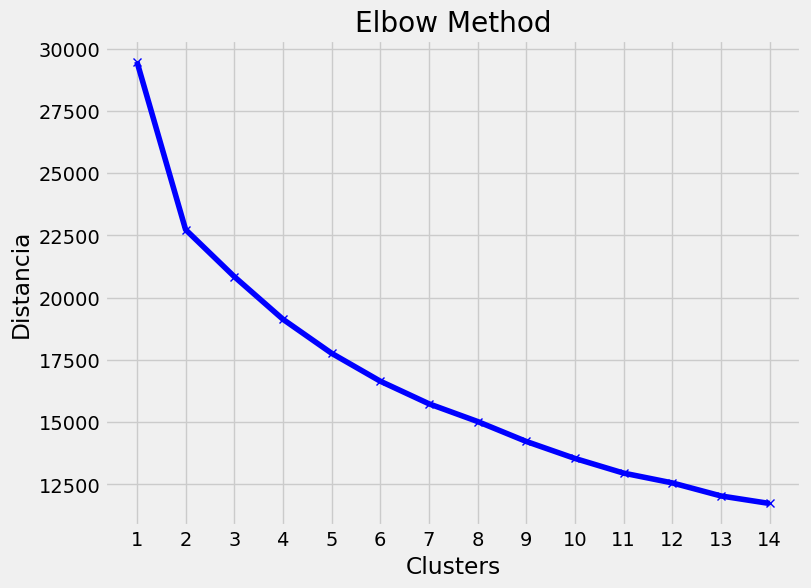
\includegraphics[scale=0.3]{/Users/ely/Documents/Maestria/segundo_semestre/cimat2023-1/patrones/Proyecto_1/imgenes/elbow.png}
		\caption{Método del codo para aproximar el número de clusters.}
		\label{elbow} 
   \end{center} 
\end{figure} 



Para ayudarnos a determinar si los datos tienen o no una estructura o se agrupan unos con otros, utilizaremos el algoritmo de k-means sobre los los datos proyectados en las tres pirmeras componentes principales. Para ello, primero nos apoyamos en el método del codo para tener una idea de donde comenzar el número de clusters.


\begin{figure} [H]
	\begin{center}
		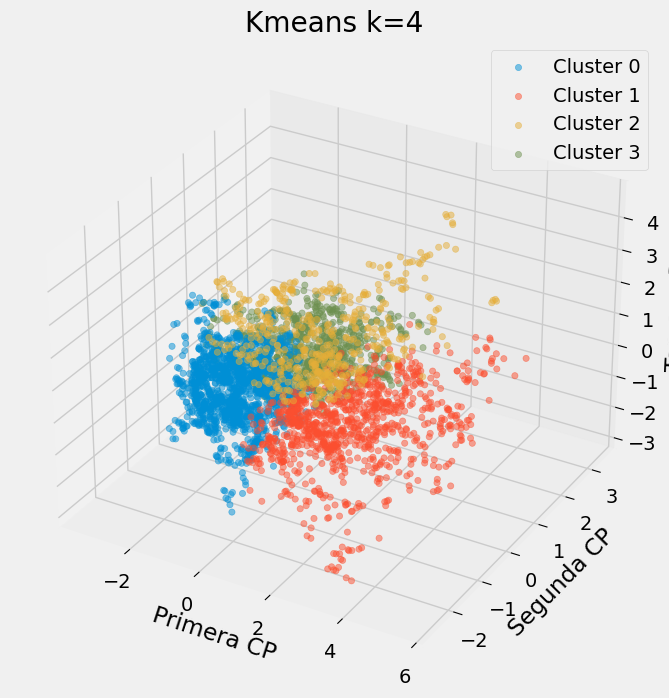
\includegraphics[scale=0.35]{/Users/ely/Documents/Maestria/segundo_semestre/cimat2023-1/patrones/Proyecto_1/imgenes/kmeans4.png}
		\caption{kmeans con 4 clusters sobre los datos reducidos a tres dimensiones}
		\label{kmeans4} 
   \end{center} 
\end{figure} 

Con base en la gráfica obtenida \ref{elbow}  con este método, decidimos comenzar con 4 clusters. En la figura \ref{kmeans4} se muestran los datos en tres dimensiones coloreados según el cluster determinado con el algoritmo k-means. 


Para saber si la clasificación del algoritmo se hizo en función de alguna de las variables categoricas que tenemos disponibles, realizamos gráficos de frecuencia para cada etiqueta del cluster y para cada variable categórica.

En la figura \ref{kmeans4anio} se encuentra el histograma de la variable año para cada uno de los cuatro clusters.
\begin{figure} [H]
	\begin{center}
		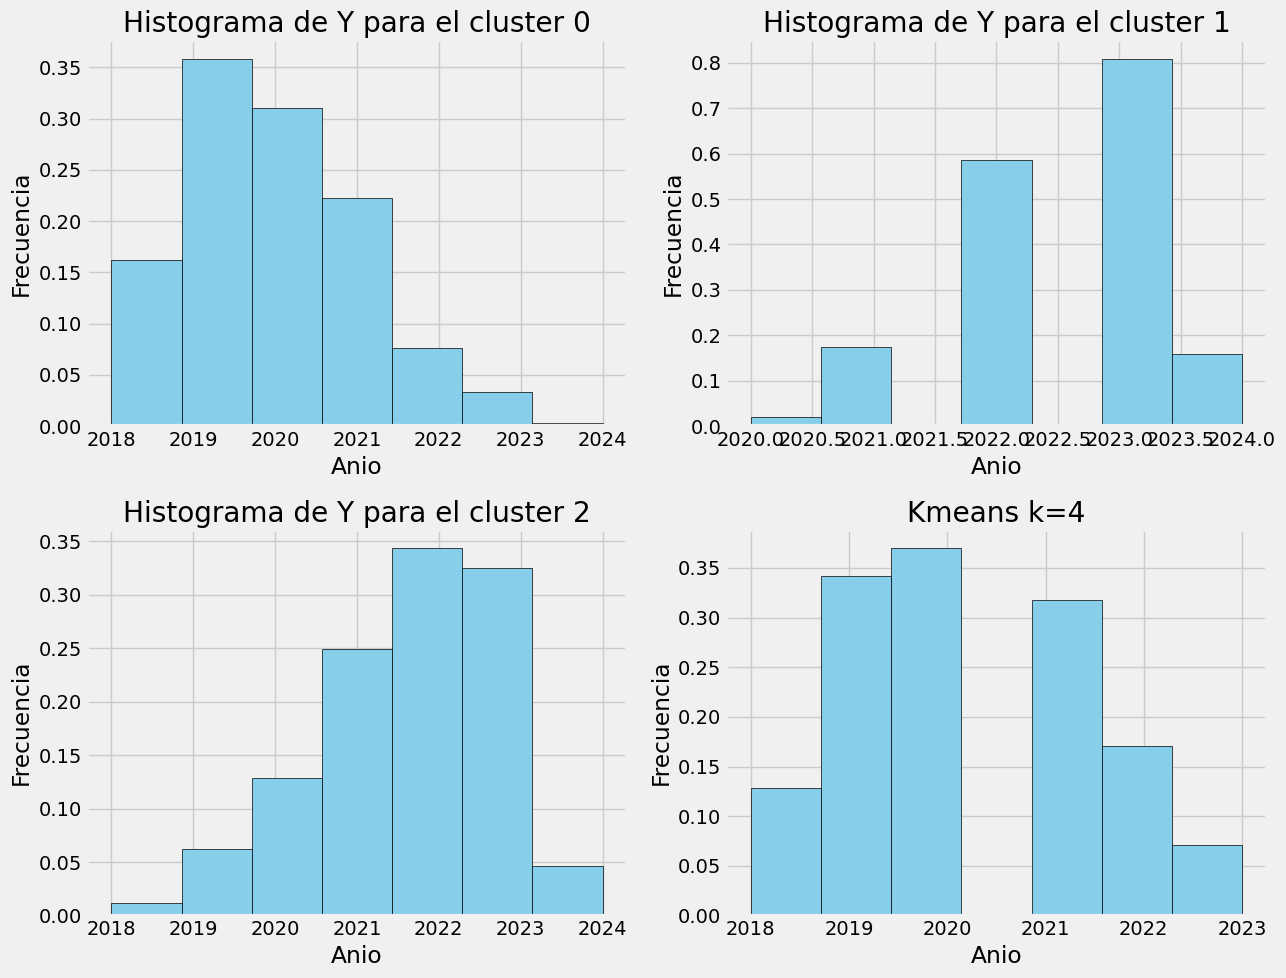
\includegraphics[scale=0.25]{/Users/ely/Documents/Maestria/segundo_semestre/cimat2023-1/patrones/Proyecto_1/imgenes/kmeans4anio.png}
		\caption{Frecuencias de cada año en por cluster. }
		\label{kmeans4anio} 
   \end{center} 
\end{figure} 


En la figura \ref{kmeans4mes} se encuentra el histograma de la variable mes para cada uno de los cuatro clusters.
\begin{figure} [H]
	\begin{center}
		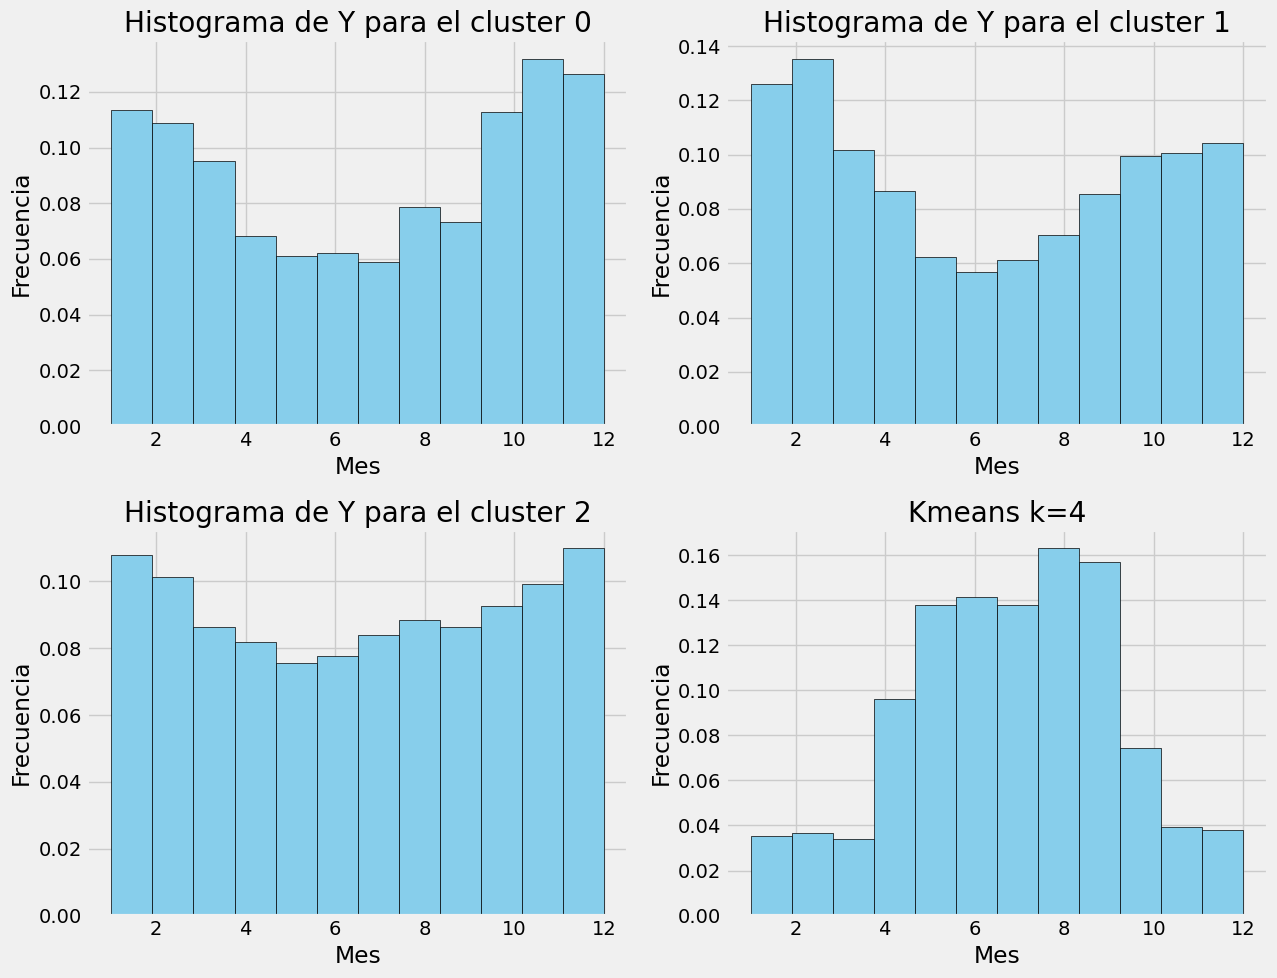
\includegraphics[scale=0.25]{/Users/ely/Documents/Maestria/segundo_semestre/cimat2023-1/patrones/Proyecto_1/imgenes/kmeans4mes.png}
		\caption{Frecuencias de cada mes en por cluster. }
		\label{kmeans4mes} 
   \end{center} 
\end{figure} 

En la figura \ref{kmeans4vat} se encuentra el histograma de la variable categoria para cada uno de los cuatro clusters.

\begin{figure} [H]
	\begin{center}
		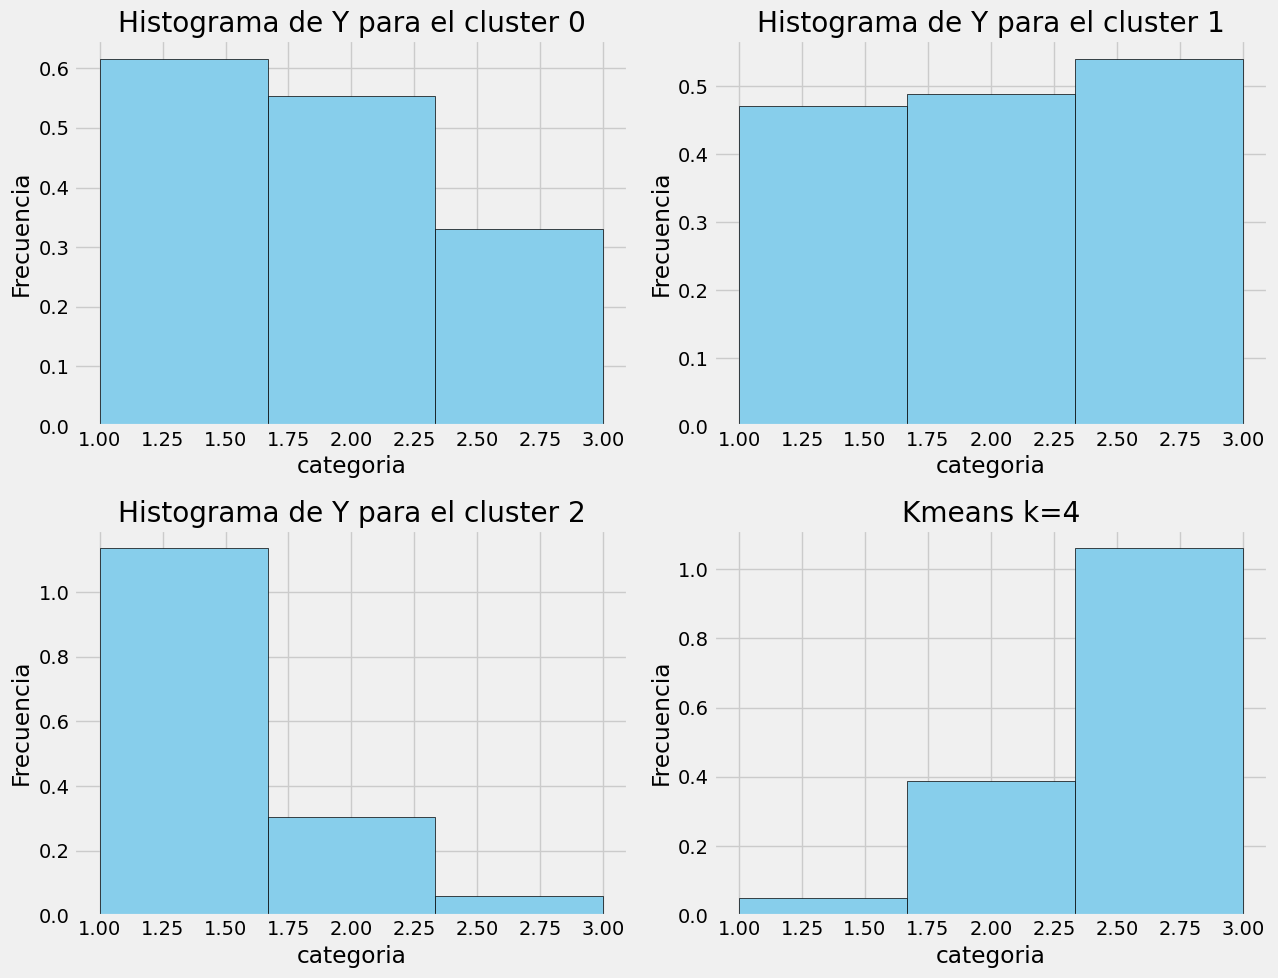
\includegraphics[scale=0.25]{/Users/ely/Documents/Maestria/segundo_semestre/cimat2023-1/patrones/Proyecto_1/imgenes/kmeans4vat.png}
		\caption{Frecuencias de cada categoria en por cluster. }
		\label{kmeans4vat} 
   \end{center} 
\end{figure} 

En la figura \ref{kmeans4season} se encuentra el histograma de la variable estación para cada uno de los cuatro clusters.

\begin{figure} [H]
	\begin{center}
		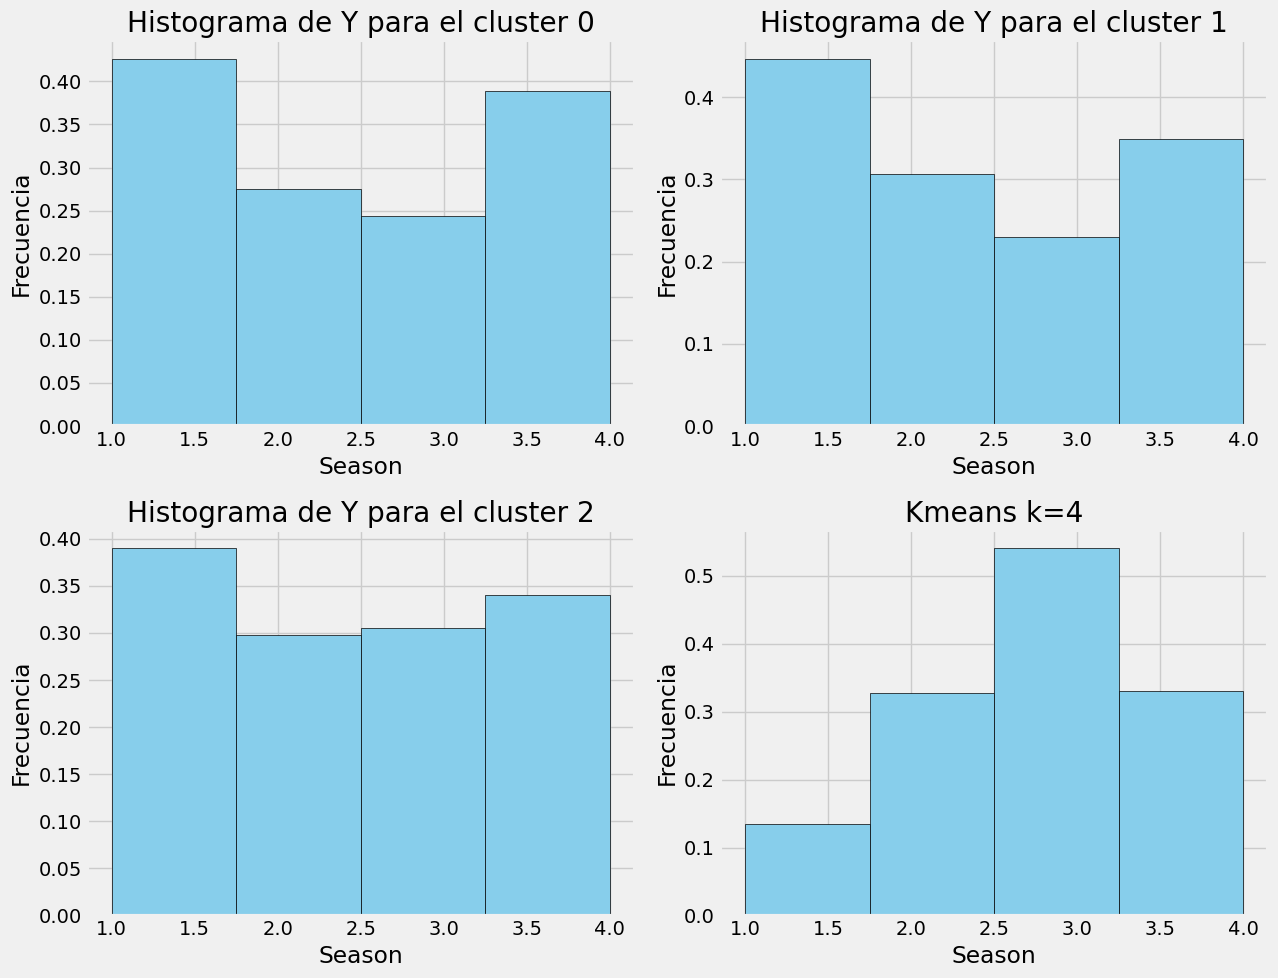
\includegraphics[scale=0.25]{/Users/ely/Documents/Maestria/segundo_semestre/cimat2023-1/patrones/Proyecto_1/imgenes/kmeans4season.png}
		\caption{Frecuencias de cada estacion en por cluster. }
		\label{kmeans4season} 
   \end{center} 
\end{figure} 



Las dos variables categóricas más discriminantes son año y categoria. Mientras que mes y estación no nos dicen mucho. En los cuatro clusters hay cantidades altas de más de una etiqueta.

Tomando en cuenta el método del codo y los histogramas anteriores se probó el algoritmo k-means para tres clusters sin embargo los histogramas son parecidos a los anteriores, y no se discierne ninguna variable discriminante.

Finalmente, como caso especial debido al aparente agrupamiento que se observa desde el gráfico de pca, se probaron 7 clusters y de igual manera se realizó el gráfico en tres dimensiones.

\begin{figure} [H]
	\begin{center}
		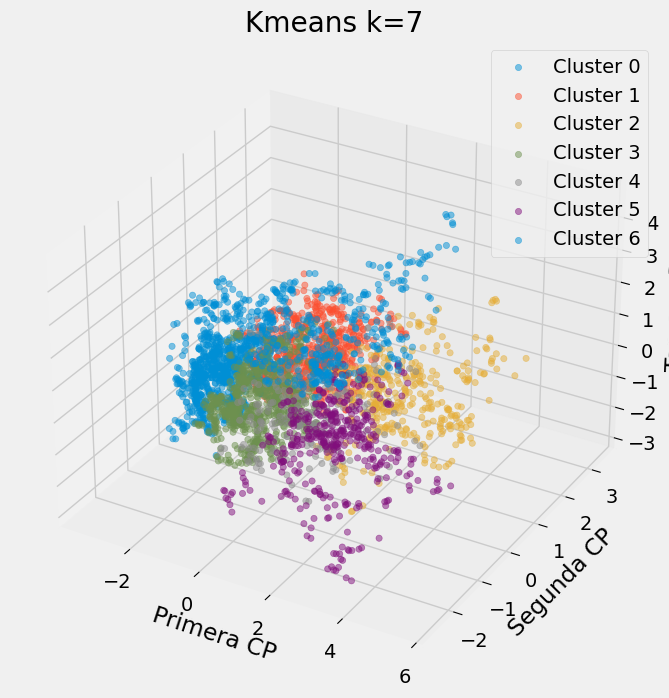
\includegraphics[scale=0.35]{/Users/ely/Documents/Maestria/segundo_semestre/cimat2023-1/patrones/Proyecto_1/imgenes/kmeans7.png}
		\caption{kmeans con 7 clusters sobre los datos reducidos a tres dimensiones}
		\label{kmeans7} 
   \end{center} 
\end{figure} 

Tal como en \ref{kmeans4} también se aprecian grupos definidos, es dificil decir si hay más traslape en uno que otro con este par de gráficos. Sin embargo en los interactivos del notebook \texttt{pca$\_$clustering.ipynb} se pueden ver desde distintas perspectivas y parecen clusters más definidos com $k=4$

\begin{figure} [H]
	\begin{center}
		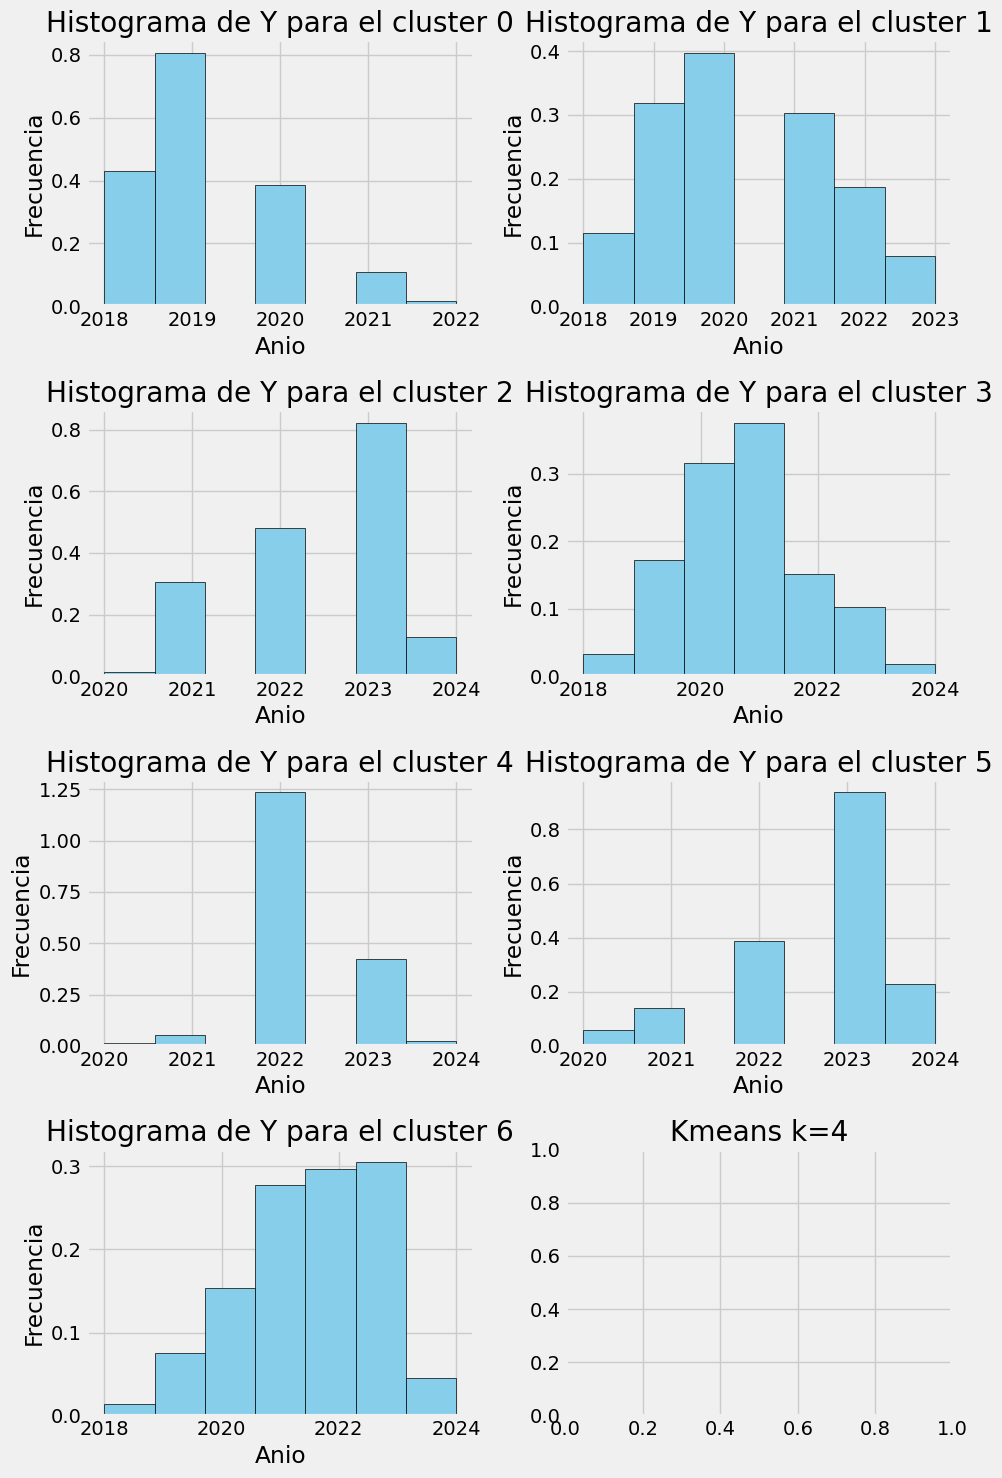
\includegraphics[scale=0.25]{/Users/ely/Documents/Maestria/segundo_semestre/cimat2023-1/patrones/Proyecto_1/imgenes/anio7.png}
		\caption{Frecuencias de cada año en por cluster.}
		\label{anio7} 
   \end{center} 
\end{figure} 



\onecolumngrid
\section{Conclusiones}
Aplicando una reducción de dimensión a nuestros datos, se puede apreciar una cierta estructura relacionada con el año de los datos. El algoritmo de agrupamiento k-means sugiere además que si una característica importante es \textit{el tipo de ciudad}. Un problema de esta clasificación es que  que engloba y resume (de manera muy sencilla) demasiados momentos en el tiempo, sería interesante hacer una clasificación de las ciudades que rescate mejor la información del tiempo.

\onecolumngrid

\section*{Referencias}

\begin{enumerate}
    \item Instituto Nacional de Estadística y Geografía (INEGI). (s/f). Precios promedio. Recuperado de \url{https://www.inegi.org.mx/app/preciospromedio/?bs=18}
    
    \item Banco de México. (s/f). Recuadros del Informe Trimestral. Recuperado de \url{https://www.banxico.org.mx/publicaciones-y-prensa/informes-trimestrales/recuadros/%7B1433DE85-D1A1-672C-CAF2-17E95DBA5BC0%7D.pdf}
\end{enumerate}



%%%%%%%%%%%%%%%%%%%%%%%%%%%%%%%%%%%%%%%%%%%%%%%%%%%%%%%%%%%%%%%%%%%%%%%%%%%%
%%%%%%%%%%%%%%%%%%%%%%%%%%%%%%%%%%%%%%%%%%%%%%%%%%%#5EJEMPLOS%%%%%%%%%%%%%
%%%%%%%%%%%%%%%%%%%%%%%%%%%%%%%%%%%%%%%%%%%%%%%%%%%%%%%%%%%%%%%%%%%%%%%%%%%%


%%%%%%%%%%%%%%%%%%%%%%%%%%%%%%%%%%%%%%%%%%%%%%%%%%%%%%%%%%%%%%%%%%%%%%%%%%%%
%%%%%%%%%%%%%%%%%%%%%%%%%%%%%%%%%%%%%%%%%%%%%%%%%%%%%%%%%%%%%%%%%%%%%%%%%%%%
%%%%%%%%%%%%%%%%%%%%%%%%%%%%%%%%%%%%%%%%%%%%%%%%%%%%%%%%%%%%%%%%%%%%%%%%%%%%

%%%%%%%%%%%%%%%%%%%%%%%%%%%%%%%%%%%%%%%%%%%%%%%%%%%%%%%%%%%%%%%%%%%%%%%%%%%%
%%%%%%%%%%%%%%%%%%%%%%%%%%%%%%%%%%%%%%%%%%%%%%%%%%%%%%%%%%%%%%%%%%%%%%%%%%%%
%%%%%%%%%%%%%%%%%%%%%%%%%%%%%%%%%%%%%%%%%%%%%%%%%%%%%%%%%%%%%%%%%%%%%%%%%%%%
%%%%%%%%%%%%%%%%%%%%%%%%%%%%%%%%%%%%%%%%%%%%%%%%%%%%%%%%%%%%%%%%%%%%%%%%%%%%



%%%%%%%%%%%%%%%%%%%%%%%%%%%%%%%%%%%%%%%%%%%%%%%%%%%%%%%%%%%%%%%%%%%%%%%%%%%%
%%%%%%%%%%%%%%%%%%%%%%%%%%%%%%%%%%%%%%%%%%%%%%%%%%%#6BIBLIOGRAFÍA%%%%%%%%%%%%%
%%%%%%%%%%%%%%%%%%%%%%%%%%%%%%%%%%%%%%%%%%%%%%%%%%%%%%%%%%%%%%%%%%%%%%%%%%%%


\end{document}
